%!TEX root = ../../main.tex

\section{CDB optimal weights} % (fold)
\label{app:cdb_weights}

% section cdb_optimal_weights (end)

\begin{figure}[htbp]
  \centering
  \footnotesize
  \renewcommand{\arraystretch}{1.2}

  \caption{CDB optimal weights with five factors}

  \begin{longcaption}
    Smoothed as 1-year moving averages. Left hand panel including and excluding HML, right hand including and excluding CMA. Based on one-week-ahead forecasts from the copula model 1963--2016.
  \end{longcaption}
  
  \begin{subfigure}{0.45\textwidth}
    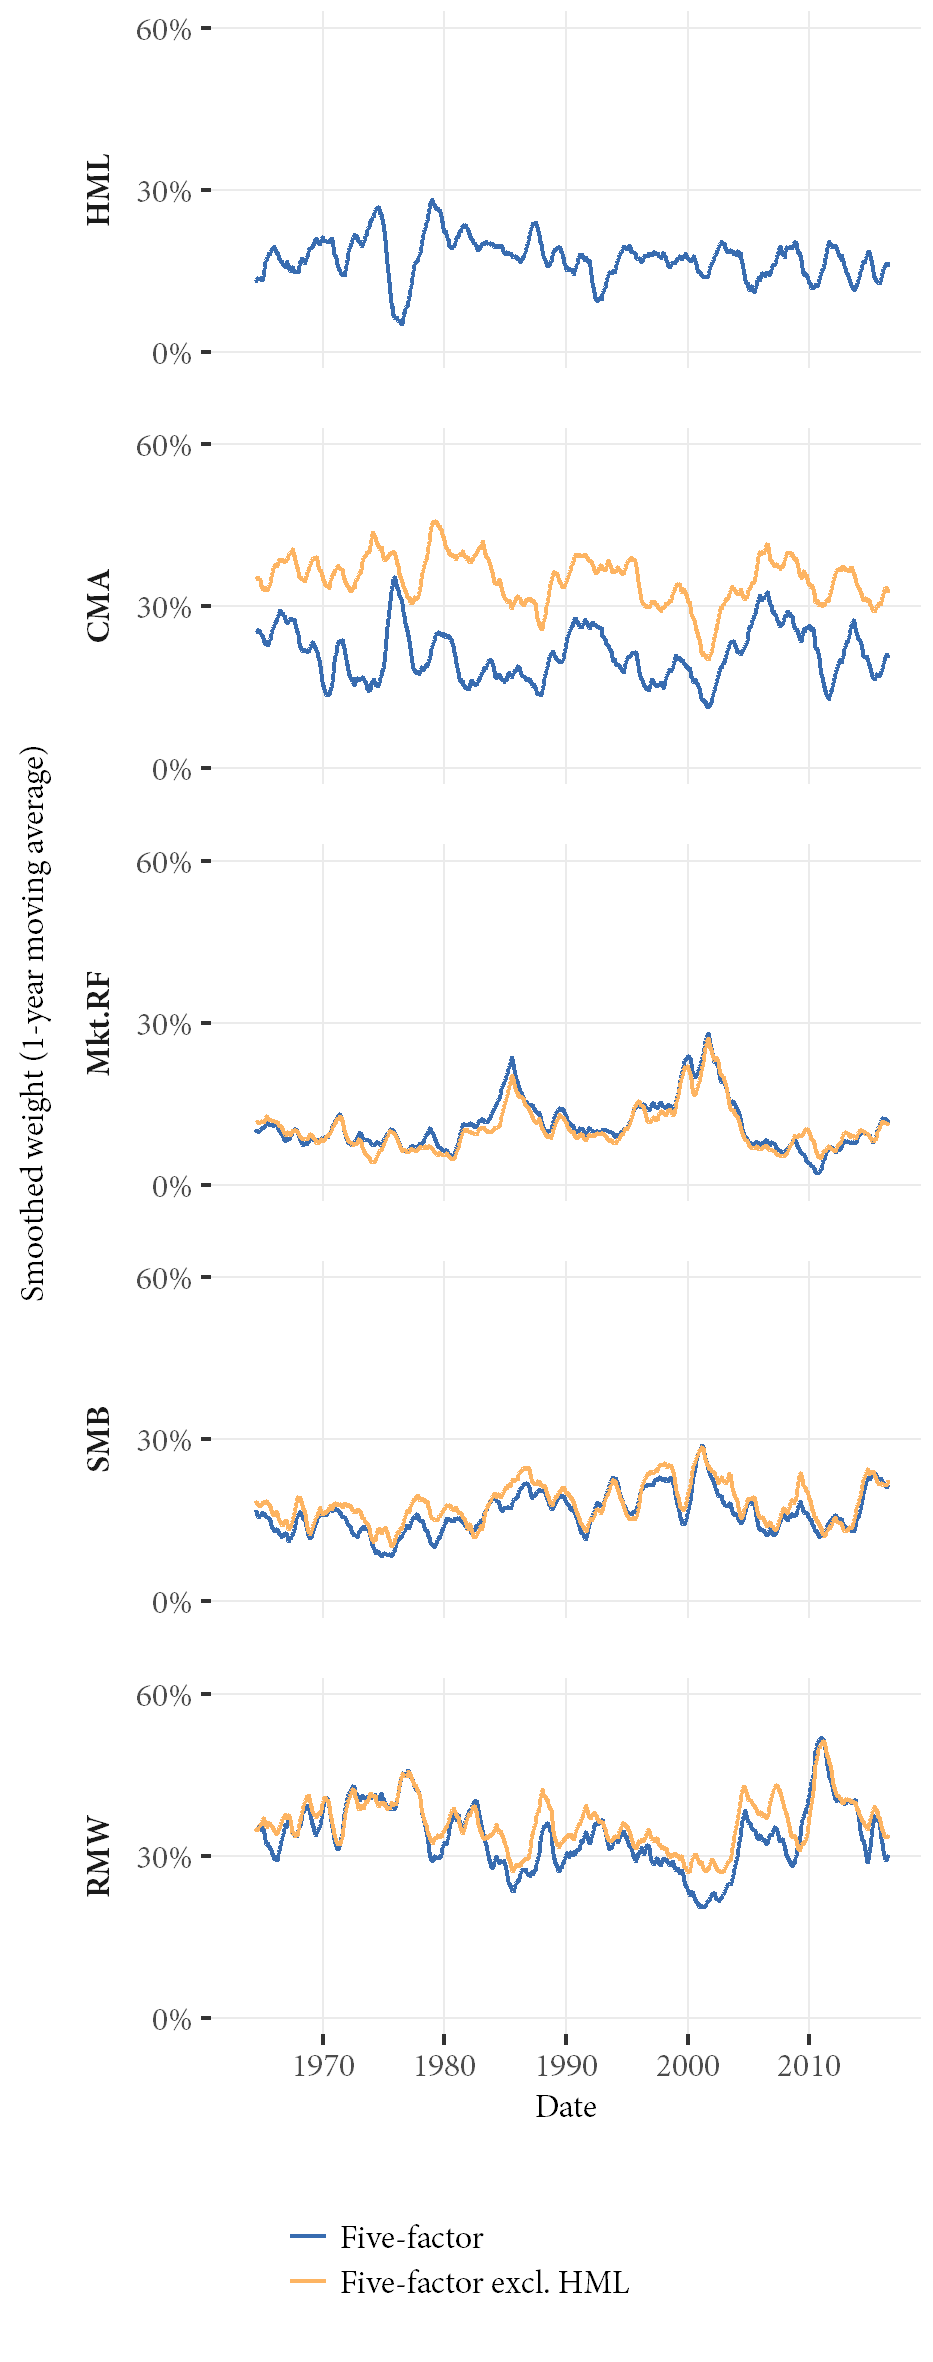
\includegraphics[width=\textwidth]{graphics/weights/appendix_Weights_CDB_5F_EXCL_HML_5F.png}
    \caption{Excluding HML}
  \end{subfigure}
  ~
  \begin{subfigure}{0.45\textwidth}
    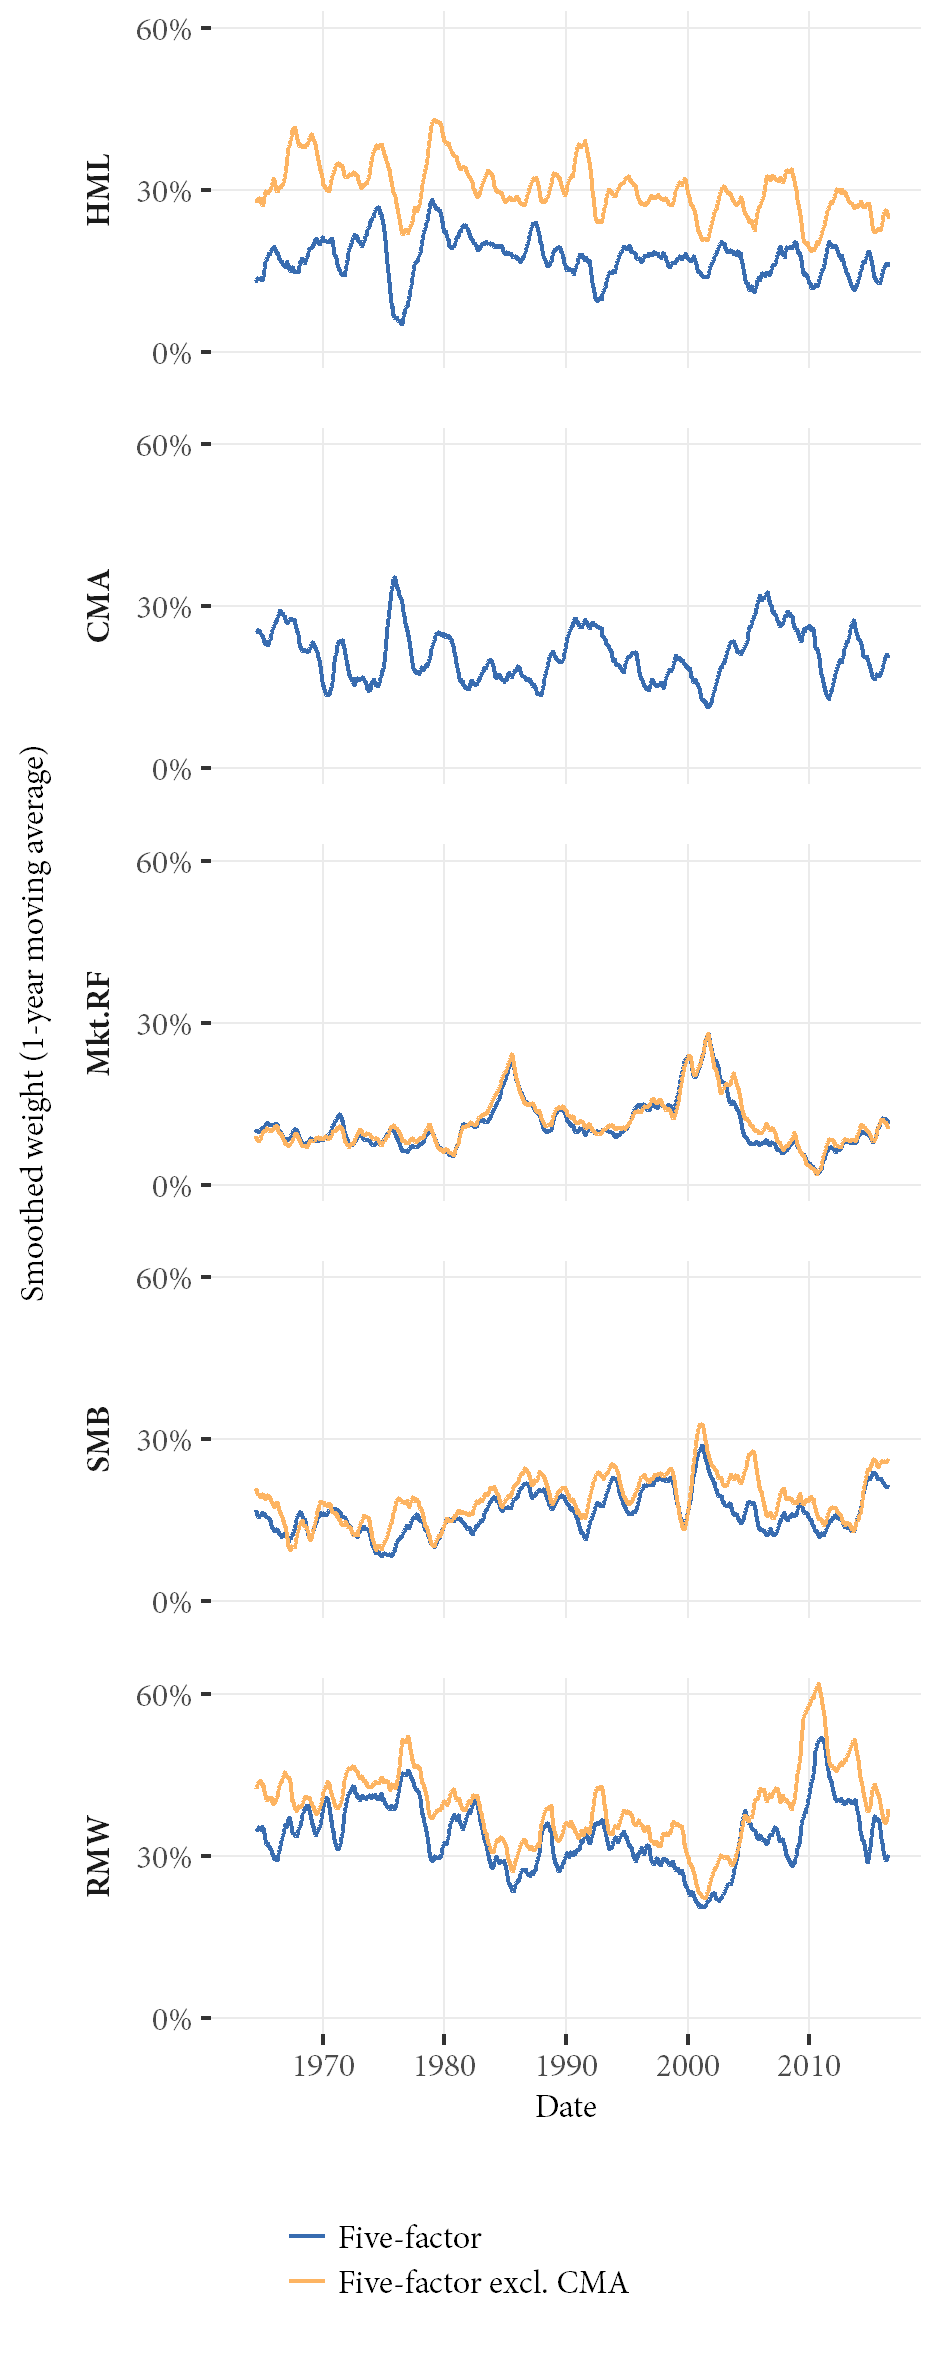
\includegraphics[width=\textwidth]{graphics/weights/appendix_Weights_CDB_5F_EXCL_CMA_5F.png}
    \caption{Excluding CMA}
  \end{subfigure}
\end{figure}

\begin{figure}[htbp]
  \centering
  \footnotesize
  \renewcommand{\arraystretch}{1.2}

  \caption{CDB optimal weights with six factors}

  \begin{longcaption}
    Smoothed as 1-year moving averages. Left hand panel including and excluding HML, right hand including and excluding CMA. Based on one-week-ahead forecasts from the copula model 1963--2016.
  \end{longcaption}

  \begin{subfigure}{0.45\textwidth}

    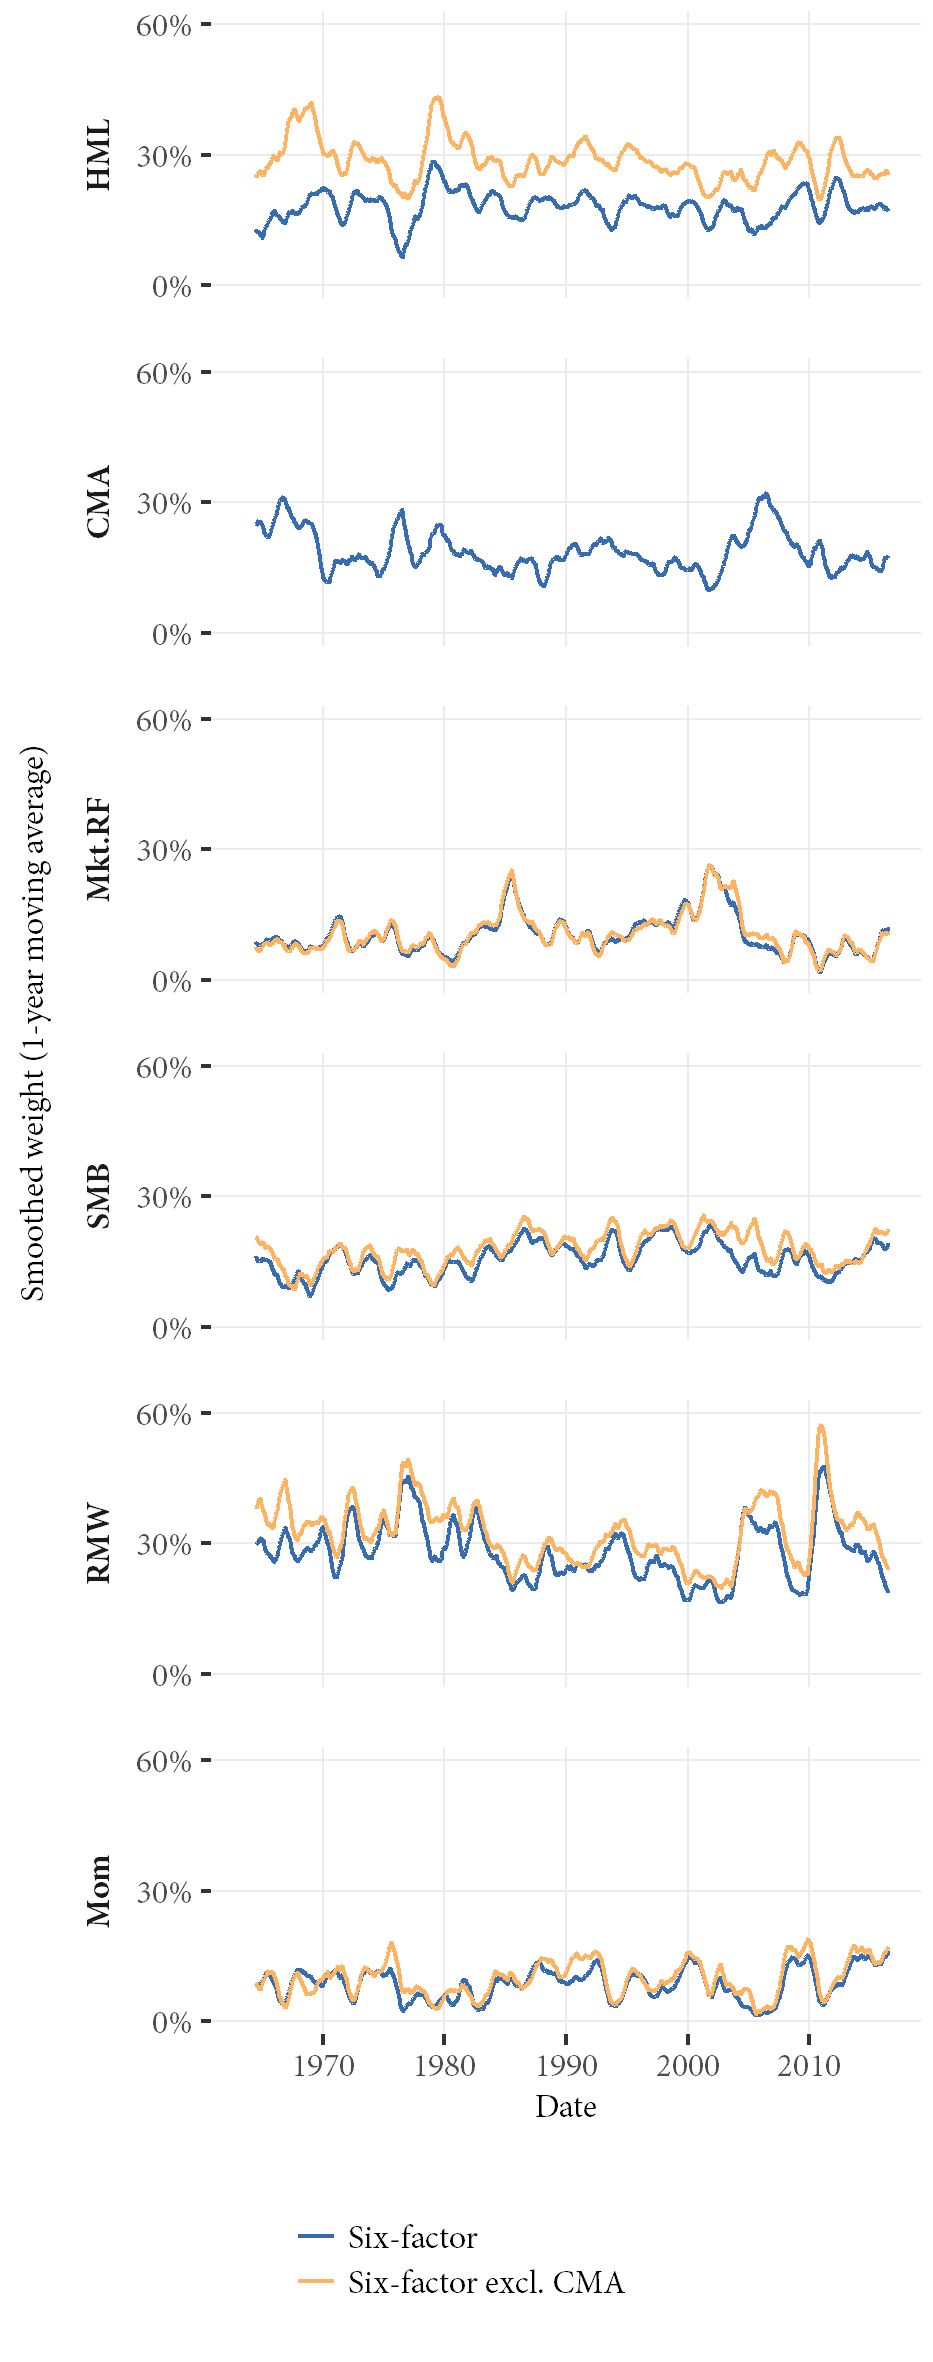
\includegraphics[width=\textwidth]{graphics/weights/appendix_Weights_CDB_6F_EXCL_CMA_6F.png}
    \caption{Excluding HML}
  \end{subfigure}
  ~
  \begin{subfigure}{0.45\textwidth}
    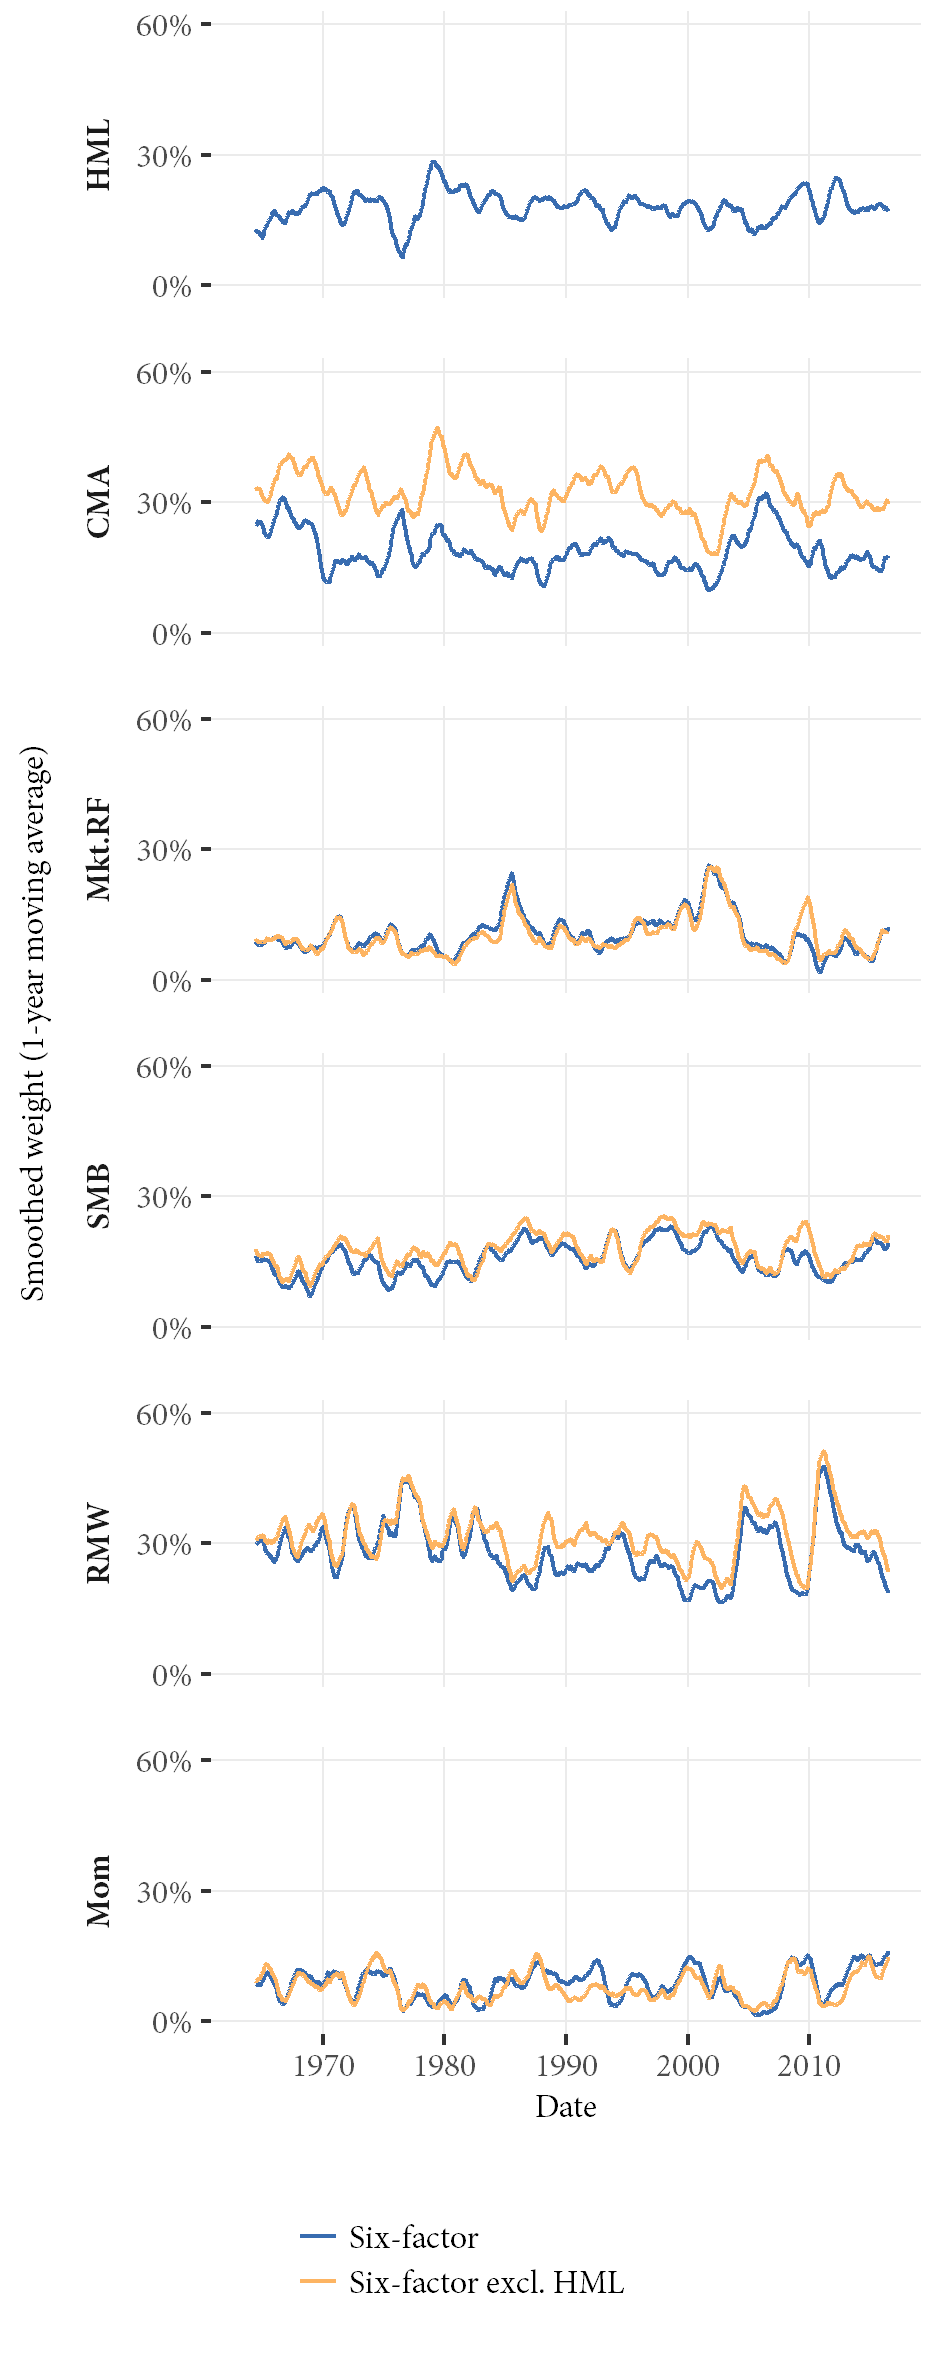
\includegraphics[width=\textwidth]{graphics/weights/appendix_Weights_CDB_6F_EXCL_HML_6F.png}
    \caption{Excluding CMA}
  \end{subfigure}
\end{figure}
